\documentclass[a4paper,10pt]{article}
\usepackage{mathtools}
\usepackage{amssymb}
\usepackage{titling}
\usepackage{lipsum}
\usepackage{graphicx}
\graphicspath{ {./images/} }
\usepackage{float}
\usepackage[hidelinks]{hyperref}
\usepackage[T1]{fontenc}

\pretitle{\begin{center}\Huge\bfseries}
\posttitle{\par\end{center}\vskip 0.5em}
\preauthor{\begin{center}\Large\ttfamily}
\postauthor{\end{center}}
\predate{\par\large\centering}
\postdate{\par}

\pretitle{\begin{center}\Huge\bfseries}
\posttitle{\par\end{center}\vskip 0.5em}
\preauthor{\begin{center}\Large\ttfamily}
\postauthor{\end{center}}
\predate{\par\large\centering}
\postdate{\par}

\title{Choosing between Containerization or Virtualization}
\author{Jonas Thorhauge Grønbek, Kristoffer Lock Tølbøll}
\date{\today}

\begin{document}
			
	\maketitle
	\thispagestyle{empty}
	
	\begin{abstract}
	Technologies like virtualization and containerization have had a major impact in software development. There seems to be some general confusion about the differences between the two and when to utilize one over the other - which could lead to inefficient or unmaintainable code-bases. We will throughout our article elaborate on the differences between the two and conclude the relevant considerations that should be taken into account before implementing either.
	\end{abstract}
	
	\section{History and origin of Containerization}
	Containerization has been around for a long time. Chroot first came out in 1979, and gave developers the ability to change the root directory of a process. This feature enables developers to encapsulate programs in a contained file system, which is isolated from the original file system. This idea was expanded upon, when Jails came out in 2000.

	Jails provides a modified runtime environment, hereby the name Jails. \cite{pii:2014}These processes are “jailed” or isolated from other processes on the host platform. Jails was the first attempt at creating a software that creates independent “mini systems” all sharing the same kernel. This is the main idea of Containerization. \\\\
	Solaris Containers were developed by Sun Microsystems, the original developer of the Java Programming language. This provided a better way to isolate processes, but these Containerization methods still required a lot of configuration and maintenance.\\\\
	Later Linux containers were introduced which was a software very similar to since it provides an OS level Virtualization technology, which can be used to either sandbox applications or to emulate an entirely new host. Docker extends upon this concept as it provides a high-level api with a single lightweight Virtualization solution to run isolated processes. 
	
	This concept of Linux Containerization is also referred to as virtual environments, which are different from Virtual Machines. In virtual environments there is no preloaded emulation manager software as there is in a Virtual Machine. This can help us optimize performance, because each isolated instance only packages the needed applications and respective dependencies. Where Virtual Machines package an entire operating system, and the underlying 
	infrastructure.\\\\
	\cite{CCC:2017}In 2013 Docker was introduced which solved a lot of the issues with regards to deploying applications on Virtual Machines and Virtual Environments as infrastructure providers. 
		\begin{figure}[H]
		\centering
		\label{marker}
		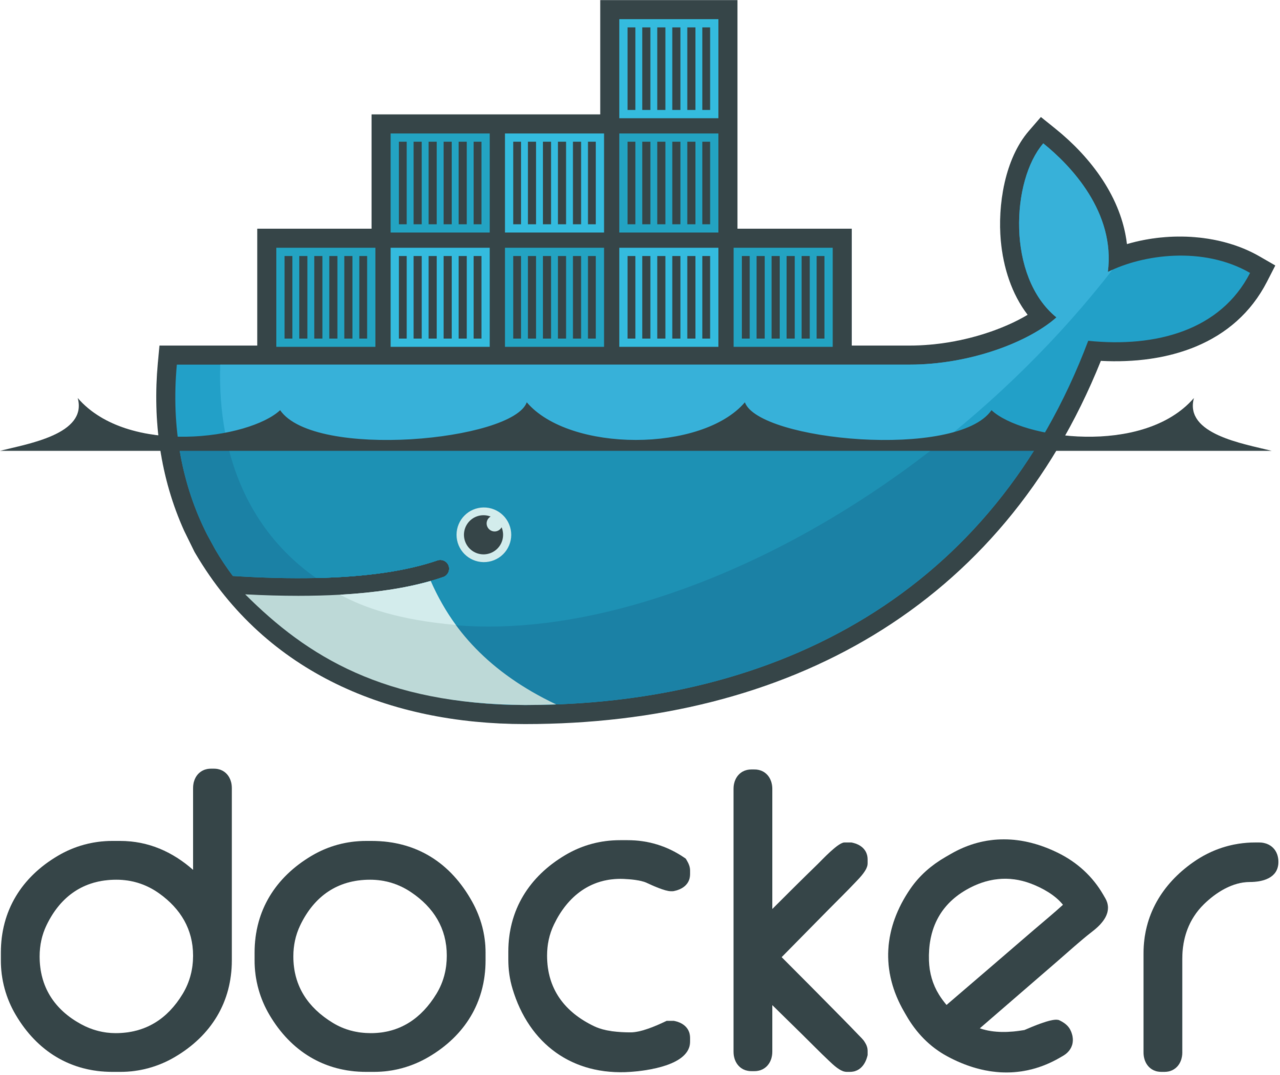
\includegraphics[width=\textwidth/2]{docker_logo}
		\caption{Docker logo}
	\end{figure}
	The etymological origin of Docker as well as the design of the logo, is an analogy of the shipping and container industry. Similar to how shipping solves the logistical issues of manually loading, unloading, protecting fragile merchandise and orchestrating different shipments between several countries and continents. 
	
	Docker solves similar issues present in the software industry with regards to manual development of containers, difficulty of isolating processes and different platforms requiring specific configurations, and dependencies.
	
	\section{Containerization in contrast to Virtualization} 
	What is the difference between Virtualization and containers?
	
	When comparing Virtualization to Containerization, Virtualization enables the user to run multiple operating systems on the hardware infrastructure of a single physical server. Virtualization is typically used in instances, where we need full functionality from the underlying operating system. This advancement in Virtualization is often seen in state of the art web applications. 
	
	When comparing Containerization to Virtualization, Containerization provides abstraction on an operating-system level and limits the resources available to the machine as per required, to run the application in the container. Virtualization is a hardware-level abstraction where we ship the entire operating system, meaning that it has its own kernel implementation. Containers share the same kernel. This also means that Virtualization provides full isolation and increased security, while containers are process level isolated which essentially provides a less secure environment. 
	
	When we think of Virtualization, the most common practise is to use Virtual Machines. As mentioned above, this is a hardware level abstraction, meaning it lays between the operating system and the physical hardware layer. 
	
	The Virtual Machine consists of the actual Virtual Machine along with a hypervisor, this is the management software that allows an Operating System to run multiple Virtual Machines sharing the same physical resources. 
	
	\begin{figure}[H]
		\centering
		\label{marker}
		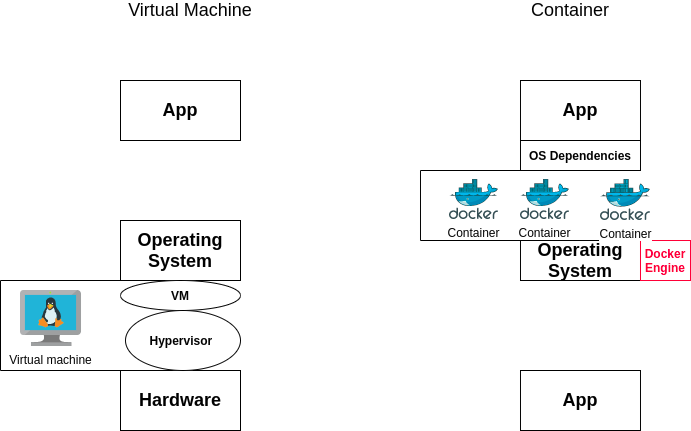
\includegraphics[width=\textwidth]{vm_container}
		\caption{Diagram illustrating the differences between Containerization and Virtualization}
	\end{figure}
	Illustrated above is the abstraction between Operating System and application. 
	By using Docker the Operating System can run several applications in containers, if utilizing Virtual Machines. The difference is, In theory these practises can be used alongside each other, as Docker containers can also run on a Virtual Machine. The Docker Engine is the technology that spins up Docker containers, and it only requires an operating system to function. It does not take the physical hardware specifications into account. Whereas a Virtual Machine, is an abstraction in between the operating system, and the physical hardware. 
	
	What is the best use case for each respective practise? 
	In regards to cloud technology and dev-ops, when do we want to use Virtualization and when do we want to use Containerization? 
	
	\section{Containerization pro’s and con’s}
	In the modern day application development landscape,
	Containerization can be a powerful technique for optimizing deployment of applications . But there are also situations, where you might not want to use it. \\\\
	Cons of using Docker:
	Containers typically rely on a base image. This could for example be a nodeJS image or a python image, if we were trying to run a web application. It could also be a centos or ubuntu image if we wanted an operating system as the base image. Depending on the situation, base images can contain vulnerabilities because they are maintained by external parties. 
	\cite{osti_1244917}
	In some use cases, there are special compliance requirements that require you to manually manage the infrastructure. In recent years, the global political landscape has had an increased focus on data compliance and security measures when storing user data. Since the GDPR (General Data Protection Rights) agreement, made by the European Union in 2016, along with multiple other regulations, has ensured that certain industries have special regulatory requirements, in terms of hardware storage and encryption. When we abstract the physical layer using Containerization and Virtualization, there are some limitations to the hardware, this means we can’t control the hardware storage. 
	\\\\
	Cons of not using Docker: 
	Without Docker we would have to manually set up a development environment for our application to function. This would mean installing and requiring dependencies, setting up configuration files, managing infrastructure etc. This would result in a necessity to set up replica environments for each new application This equates to less scalability, decreased security and a longer more complicated setup process giving higher error and misconfiguration margins\\\\
	To elaborate on the first issue, a similar issue arises when we utilize multiple environments for our application. We might have multiple different environments, eg: development, staging, production etc. These would each require individual maintenance and configuration, by the time we move from development or staging into a production environment, the dependencies may be outdated, this could result in ending up with a different version than our intended environment. 
	Unlike Docker that provides us with an easy way to spin up, stop, and restart containers. We have no simple way of running these commands with Virtual Machines as we would have to start and stop the actual Virtual Machines, not just the application environment. 
	Without Docker we are less flexible in terms of moving and reproducing our environment. Setting up and configuring environments poses some obstacles. If we migrate to a new cloud provider or a new platform, it might be a slow and inefficient process. Because Docker is platform agnostic, it provides us a simple interface to connect to the underlying platform. 
	
	
	\section{Conclusion}
	As elaborated on throughout the article, the technology and specific use-case indicates whether to implement your software over Containerization or Virtualization. Each of the respective paradigms each provides specific circumstances to run software, and the conditions determines whether contained or virtual environments is appropriate. 
	
	If your hosted processes requires hardware access, then a Virtual Environment would be the obvious choice. Other relevant considerations could include concerns in regard to interactions, management and deployment. Containerization is the light-weight more performance oriented solution and specifically docker containers are the backbone for a lot of modern and current tools relevant to CI/CD and orchestration. If any of that is desired - then docker is the obvious choice. Should your software however require to function within it's own individual segregated OS, then Virtualization is probably to be chosen.
	
	\bibliographystyle{unsrt}	
	\bibliography{references}
\end{document}

